\documentclass[12pt, letterpaper]{article}
\usepackage[utf8]{inputenc}
\usepackage{amsfonts, amsmath, amssymb}
\makeatletter
\makeatother
\usepackage[hidelinks]{hyperref}
\usepackage{comment}
\usepackage{fullpage}
\usepackage[english]{babel}
\usepackage{pdfpages}
\usepackage{tikz}
\usepackage{graphicx}
\usepackage[colorinlistoftodos]{todonotes}
\usepackage[linesnumbered]{algorithm2e}
\usepackage{tabularx}
\usepackage{url}
\usepackage{hyperref}
\hypersetup{colorlinks=true}
\usepackage{multirow}
\usepackage[margin=0.5in]{geometry}
\usepackage[english]{babel}
\usepackage{mathtools}
\usepackage{booktabs}
\usepackage{physics}
\usepackage{enumitem}

\usepackage[thmmarks, thref]{ntheorem}

\theoremstyle{nonumberplain}
\theorembodyfont{\upshape}
\theoremseparator{.}
\theoremsymbol{\ensuremath{\square}}
\theoremsymbol{\ensuremath{\blacksquare}}
\newtheorem{sol}{Solution}
\theoremseparator{. ---}
\theoremsymbol{\mbox{\texttt{;o)}}}
\newtheorem{varsol}{Solution (variant)}

\DeclarePairedDelimiter\ceil{\lceil}{\rceil}
\DeclarePairedDelimiter\floor{\lfloor}{\rfloor}

\usetikzlibrary{matrix}
\setlength{\marginparwidth}{2cm} 

\title{MATH 4640 Numerical Analysis - HW 1 Solutions}

\author{Austin Barton}

\begin{document}
\maketitle

\vspace{2em}

\hspace{18pt}\textbf{Problem 1:} \medskip
\begin{sol}
	\begin{enumerate}[label=\roman*.]
		\item
		      \begin{enumerate}[label=\alph*)]
			      \item $2^4 * 1 + 2^3 * 1 + 2^2 * 1 + 2^1 * 0 + 2^0 * 1 + 2^{-1} * 1 + 2^{-2} * 0 + 2^{-3} * 1 + 2^{-4} * 1 + 2^{-5} * 1 = 16 + 8 + 4 + 1 + 0.5 + 0.125 + 0.0625 +  0.03125 = 29.71875$
			      \item $16^2 * 2 + 16^1 * 11 + 16^0 * 3 + 16^{-1} * 15 + 16^{-2} * 15 = 512 + 176 + 3 + 0.9375 + 0.05859375 = 691.99609375$
			      \item $\sum_{i = 1}^n 2^{i-1} * 1$
			      \item $\sum_{i = 1}^n 2^{-i} * 1$
		      \end{enumerate}
		\item
		      \begin{enumerate}[label=\alph*)]
			      \item This is $2^5 + 2^4 + 2^2 + 2^1$ so this is $11110$ in binary.
			      \item This is $2^7 +2^6 + 2^5 + 2^4 + 2^3$
			      \item First, $1_{10} = 1_2$ and $7_{10} = 111_2$. From here on, our numbers will be in base 2 (binary) representation.

			            Here we implement the long division algorithm on $\frac{1}{111}$. Consider,

			            \begin{gather*}
				            111\overline{\smash)1.000000000} \\
			            \end{gather*}

			            $111$ is larger than $1$, let our answer be $0$ currently. Now carry a $0$ from $1.000$ and consider $10/111$. $111$ is larger than $10$ so let our answer be $0.0$ currently. Now carry a $0$ from $1.000$ and consider $100/111$. $111$ is larger than $100$ so let our answer be $0.00$ currently. Now carry a $0$ from $1.000$ and consider $1000/111$. $111$ divides $1000$ by $1$ plus a remainder. Let our answer currently be $0.001$ and take $1000 - 111 = 1$ to be our remainder.

			            Repeat this process and the result is $0.\overline{001}$.

			            Hence, $1/7 = 0.\overline{001}_2$.
		      \end{enumerate}
	\end{enumerate}
\end{sol}

\newpage

% DONE
\hspace{18pt}\textbf{Problem 2:} \medskip
\begin{sol}
	\begin{enumerate}[label=\alph*)]
		% (a)
		\item Absolute error is
		      \begin{gather*}
			      |10451.0023 - 10451.001| = 0.0013
		      \end{gather*}
		      Relative error is
		      \begin{gather*}
			      \frac{0.0013}{10451.0023} = .124389983 \times 10^{-6}
		      \end{gather*}
		      % (b)
		\item Absolute error is
		      \begin{gather*}
			      |0.451011 \times 10^4 - 0.451010\times 10^4| = 0.01
		      \end{gather*}
		      Relative error is
		      \begin{gather*}
			      \frac{0.01}{0.451011\times 10^4} = 0.22171 \times 10^{-5}
		      \end{gather*}
		      % (c)
		\item $x_T = x_A + \epsilon$. Solving for $\epsilon$, $\epsilon = x_T - x_A = 10451.0023 - 10451.001 = 0.0013$.

		      $y_T = y_A + \eta$. Solving for $\eta$, $\eta = y_T - y_A = 4510.11 - 4510.10 = 0.01$.

		      $E_{rel}(x_Ay_A) = | \frac{x_A\eta + y_A\epsilon + \epsilon \eta}{x_Ty_t} | = \Big|  \frac{10451.001 \times 0.01 + 4510.10 \times 0.0013 + 0.0013 \times 0.01}{10451.0023 \times 4510.11} | = \frac{110.373153}{47135169.983253} = 0.0000023416 = 0.23416\times 10^{-5}$.

		      $x_Ay_A = 47135059.6101$.

		      In this calculation, we see that the number of accurate digits retained is $5$, which is the number of digits of the relative error in this calculation.

		      Now, $E_{rel}(x_A - y_A) = 10451.001 - 4510.10 = 5940.901$. And $x_T - y_T = 5940.8923$.

		      Thus,
		      \begin{gather*}
			      E_{rel}(x_A - y_A) = \frac{|(x_A - y_A) - (x_T - y_T)|}{x_t - y_t}  = \frac{|5940.901 - 5940.8923|}{5940.8923} \\
			      = \frac{0.0087}{5940.8923} = 0.0000014644 = 0.14644 \times 10^{-5}
		      \end{gather*}

		      In this calculation, we see that the number of accurate digits is $4$.
	\end{enumerate}
\end{sol}

\newpage

\hspace{18pt}\textbf{Problem 3:} \medskip
\begin{sol}
	NOTE TO READER: I am adjusting some basic notation to match the code I have written for these algorithms. It's not necessary but it makes it easier to reference code from the mathematical algorithm. The code for these implementations is in the `hw1.zip` file which contains the Rust package as well as a `README.md` and `Dockerfile` to help get it running.
	\begin{enumerate}[label=\alph*)]
		\item Algorithm

		      Let $B$ be the base 2 number represented in $\beta$ notation. That is, $B = (a_0 a_1 \ldots a_{l-1}.b_1 b_2 \ldots b_r)_\beta$. Note that our indices are different than the textbook, but it's the same notation nonetheless.

		      For bits to the left of the radix point do the following steps: (Note that following our notation, $l$ is the number of bits left of the radix point)

		      Let $i\in \{0, \ldots, l-1\}$. Calculate the sum $L = \sum_{i=0}^{l-1}2^{l - (i+1)}$.

		      For bits to the right of the radix point do the following steps: (Note that following our notation, $r$ is the number of bits right of the radix point)

		      Let $j\in \{1, \ldots, r\}$. Calculate the sum $R = \sum_{j=1}^r 2^{-(i+1)}$.

		      The sum, $L+R$ and that is the decimal equivalent. That is, $B = L+R$ where $B$ is the base 2 encoded number and $L+R$ is the decimal equivalent.

		      Note that all operations and numbers in the algorithm is assumed to be represented in base 10, but the algorithm remains the same nonetheless, so long as we understand our representation of the number of two ($10$ in base 2 and $2$ in base 10).

		      Thus, our algorithm takes a binary encoded number (base 2) and converts to the decimal equivalent, $L+R$.


		\item Algorithm

		      Let $D$ be the base 10 number represented in $\beta$ notation. That is, $D = (a_0 a_1 \ldots a_{l-1}.b_1 b_2 \ldots b_r)_\beta$. Note that our indices are different than the textbook, but it's the same notation nonetheless.

		      For digits to the left of the radix point do the following steps: (Note that following our notation, $l$ is the number of digits left of the radix point)

		      Let $L = ()_2$ be our current binary representation of $(a_0\ldots a_{l-1})_{10}$ at the beginning of our algorithm. Let $i\in \{0, \ldots, l-1\}$ and let $j = l-1$. While $a_1,\ldots, a_j \neq 0$ do the following:

		      If $a_0, \ldots, a_{j}\neq 0$, then prepend $a_j\mod 2$ to $L$. For $j = l-1$, we would set $L$ equal to $a_{l-1}\mod 2$. And for $j = l-2$, we would set $L$ equal to $(a_{l-2}\mod 2 a_{l-1}\mod 2)$, and so on.

		      For digits to the right of the radix point do the following steps: (Note that following our notation, $r$ is the number of digits right of the radix point)

		      Let $R = ()_2$ be our current binary representation of $(b_1 \ldots b_r)$. Now, take $(.b_1 \ldots b_r)$ (notice the radix point is included here) and apply the following algorithm:

		      Let $j = 1$. Multiply $(.b_j \ldots b_r)_{10}$ by $2$. If the radix point shifts to the right of $b_j$, then truncate and split to $(b_{j})_{10}$ and $(.b_{j+1}\ldots b_r)_{10}$. Push (append) $R$ with $1$ if $(b_j)_{10}$ is equivalent to $1$ and $0$ otherwise and set $j = j+1$.

		      Repeat the previous algorithm until $(.b_j\ldots b_r)\leq 0$ or $j > r$.

		      At this point in our complete algorithm, we have a binary representation, $L$, of the digits $(a_0, \ldots, a_{l-1})_{10}$ and a binary representation, $R$, of $(b_1 \ldots b_r)_{10}$.

		      Prepending $.$ to $R$ we now have a binary representation of $(.b_1\ldots b_r)_{10}$.

		      We now concatenate $L$ and $R$ now, which we represent by $L+R$.

		      The sum, $L+R$ and that is the binary equivalent. That is, $D = L+R$ where $D$ is the base 10 encoded number and $L+R$ is the binary equivalent.

		      Thus, our algorithm takes a decimal encoded number (base 10) and converts to the binary equivalent, $L+R$.



	\end{enumerate}
\end{sol}

\newpage
\hspace{18pt}\textbf{Problem 4:} \medskip
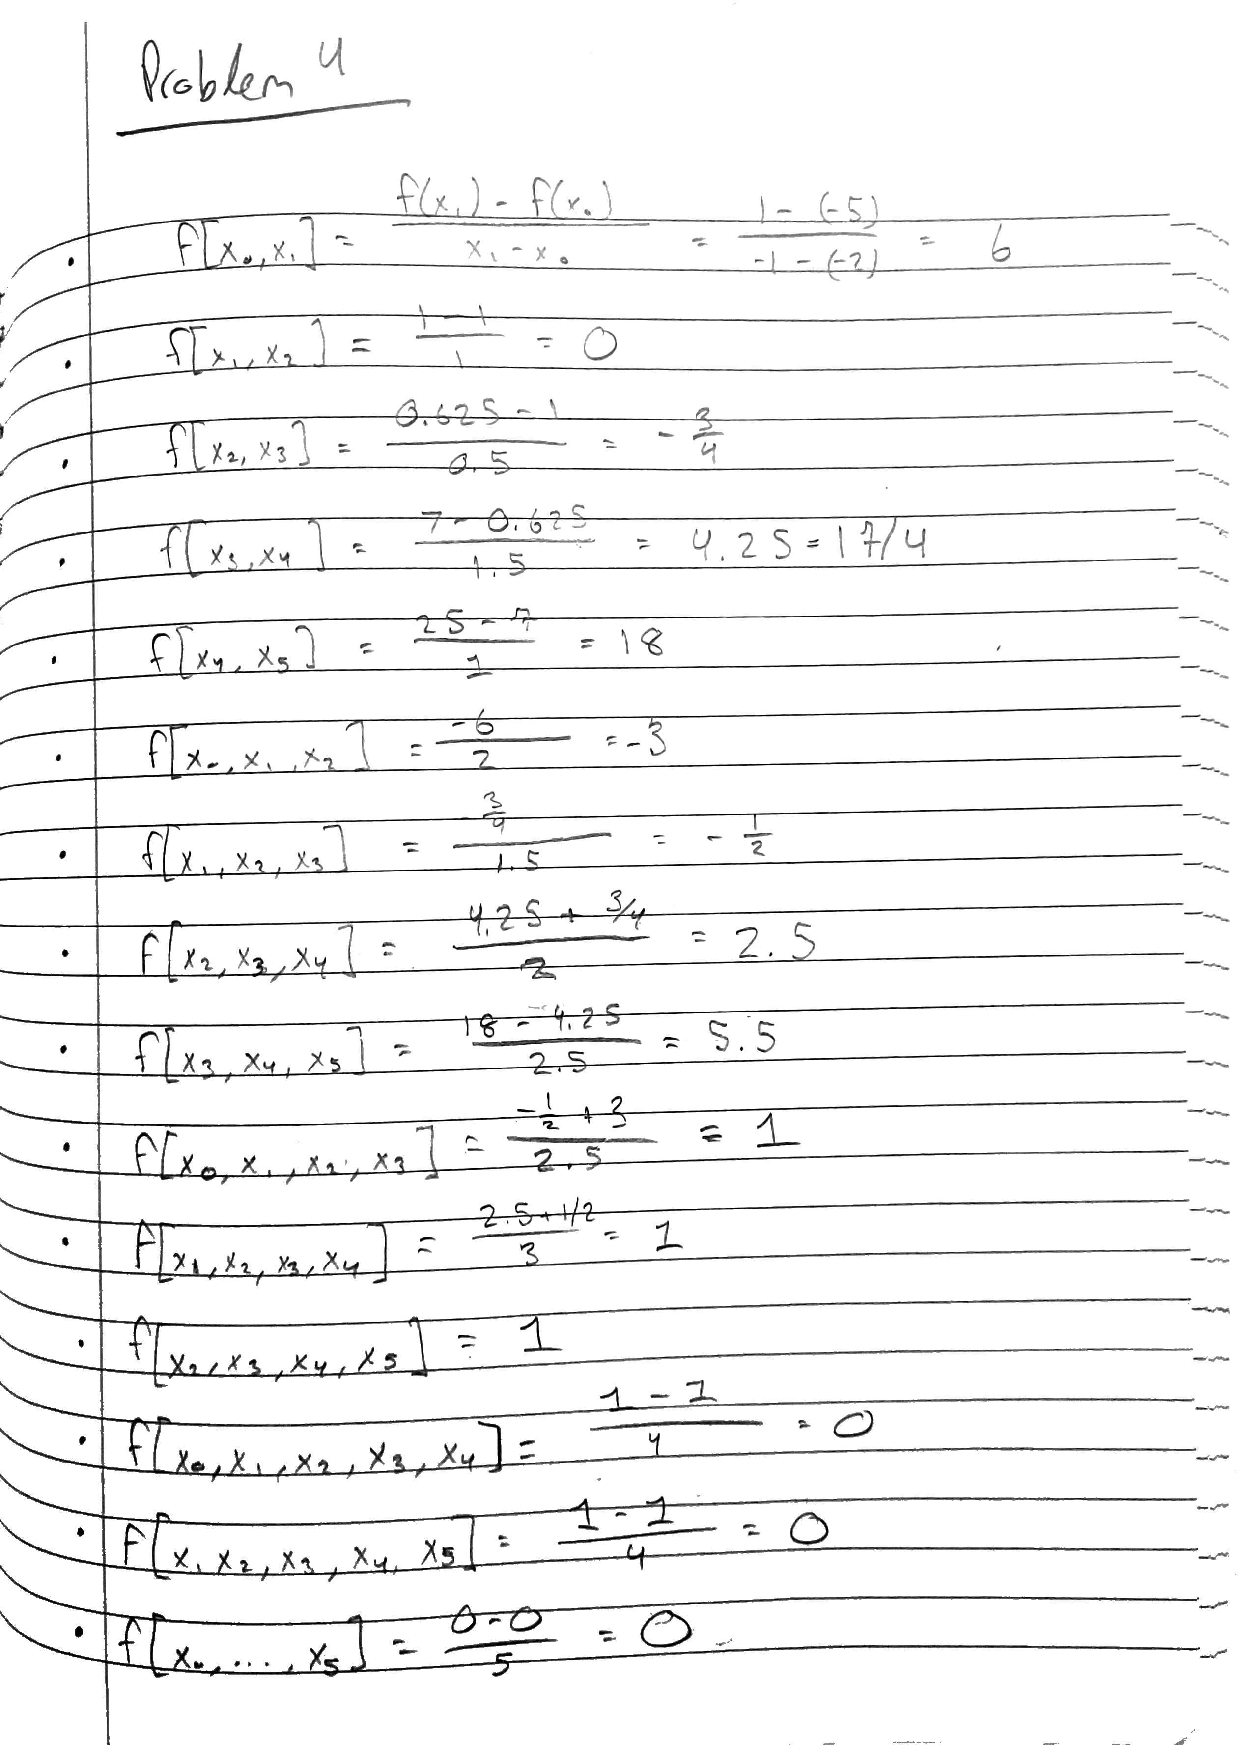
\includepdf[pages=-, scale=0.85]{4640_hw1_q4.pdf}

\hspace{18pt}\textbf{Problem 5:} \medskip
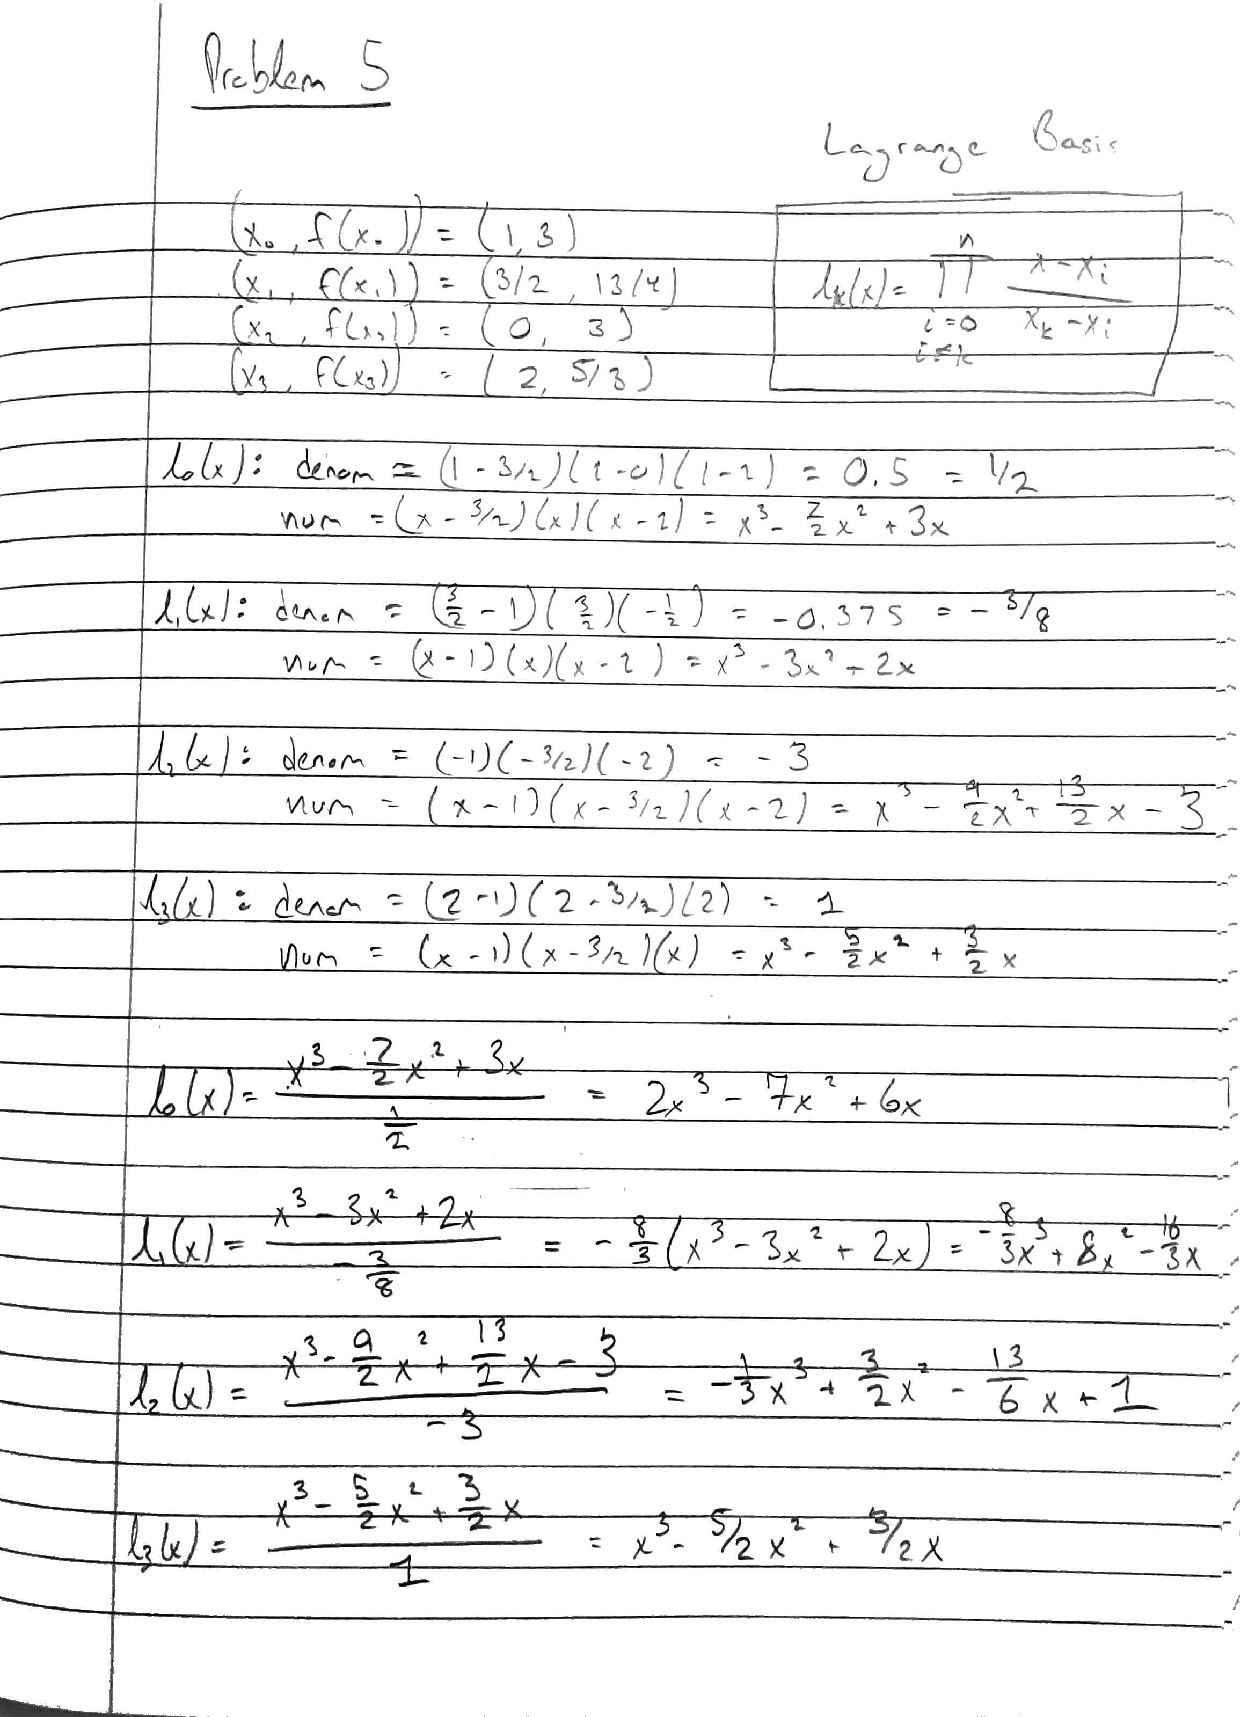
\includepdf[pages=-, scale=0.85]{4640_hw1_q5.pdf}

\newpage

\hspace{18pt}\textbf{Problem 6:} \medskip
\begin{sol}
	First, we will provie the existence of such a polynomial using Lagrange interpolation.

	In lecture we showed that, in general, give $n+1$ distinct points that the interpolation polynomial defined by
	\begin{gather*}
		p_n(x) = \sum_{k=0}^n l_k(x) f(x_k)
	\end{gather*}
	where $l_k(x) = \prod_{i=0; i\neq k}^n \frac{x - x_i}{x_k - x_i}$, interpolates the $(n+1)$ points. Additionally, $p_n(x)$ is a polynomial of degree $n$ or less.

	In case using the lecture as reference is not sufficient for grading purposes, I will provide an existence proof as follows:

	\textbf{Existence}

	Let $P_n(x)$ denote the set of polynomials of degree $\leq n$. We will show that $\exists p(x) \in P_n(x)$ such that $p(x_i) = f(x_i)$ for all $i = 0, 1, \ldots, n$.

	Consider the Lagrange interpolation formula from above. Each $l_i(x)$ is of degree $n$, and the full sum is a sum of $n$ degree polynomials, some of which (for some exponent $j$) may sum to $0$ and "cancel out". Hence, the polynomial of degree is $\leq n$.

	Now we wish to show that $p_n(x)$ interpolates $f(x)$ at each $x_i$. Recall
	\begin{gather*}
		l_k(x_i) =
		\begin{cases}
			1 & k = i    \\
			0 & k \neq i
		\end{cases}
	\end{gather*}

	So, $p_n(x_i) = \sum_{k=0}^n f(x_k)l_k(x_i) = f(x_i)l_i(x_i) + \sum_{k=0;k\neq i}^n f(x_k)l_x(x_i)$.

	But $f(x_i)l_i(x_i) = f(x_i)$ and $\sum_{k=0;k\neq i}^n f(x_k)l_k(x_i) = \sum_{k=0;k\neq i}^n f(x_k)\cdot 0 = 0$.

	Hence, $p_n(x_i) = f(x_i)$ for each $i = 0, 1, \ldots, n$. Therefore, $p_n(x)$ interpolates $f(x)$ at each $x_0, x_1, \ldots, x_n$.

	\medskip

	\textbf{Uniqueness}

	Now, we wish to provie the uniqueness of this interpolating polynomial.

	Suppose that there exists two distinct polynomials $p(x)$ and $q(x)$ of degree $\leq n$ that both interpolate the function $f(x)$ at the points $x_0, x_1, \ldots, x_n$. We want to show that $p(x) = q(x)$ for all $x$.

	Consider, $p(x) - q(x)$. This is a polynomial of degree $\leq n$.

	Now consider, $p(x_i) - q(x_i)$ for any $x_i$ where $i \in \{0, 1, \ldots, n\}$. Since $p(x)$ and $q(x)$ are both interpolating polynomials of $f(x)$, $p(x_i) - q(x_i) = f(x_i) - f(x_i) = 0$. Thus, $p(x_i) - q(x_i)$ has at least $n+1$ distinct roots, $\{x_0, x_1, \ldots, x_n\}$.

	But $p(x) - q(x)$ is a polynomial at most degree $n$ yet it has at least $n+1$ distinct roots. Therefore, $p(x) - q(x) = 0$ for all $x$. Hence, $p(x) = q(x)$ for all $x$.

	This shows that the interpolating polynomial of $f(x)$ is unique.

\end{sol}

\newpage

\hspace{18pt}\textbf{Problem 7:} \medskip
\begin{sol}
	We are given a function $f(x)$. We know that there exists a unique interpolating polynomial $p_{k}(x)$ of degree at most $k$, which interpolates $f(x)$ at the points $x_0, x_1, \dots, x_k$. That is, $f(x_i) = p_k(x_i)$ for all $i = 0, \ldots, k$.

	We want to show that
	$$f[x_0, \dots, x_k] = \frac{f^{(k)}(\xi)}{k!}$$
	for some $\xi \in (a, b)$.

	Define the error function,

	$$e_k(x) = f(x) - p_k(x)$$

	Since $p_k(x)$ is the unique polynomial of degree $\leq k$ that interpolates $f(x)$ at $x_0, \dots, x_k$, we know that

	$$e_k(x_i) = f(x_i) - p_k(x_i) = 0, \quad \text{for } i = 0, \dots, k$$

	This means that $e_k(x)$ has at least $k+1$ distinct roots at $x_0, x_1, \ldots, x_k$.

	Rolle’s Theorem states that if a function is continuous on $[a, b]$ and differentiable on $(a, b)$, and if it has two equal values at different points (i.e., $g(x_0) = g(x_1)$), then there exists some $\xi$ in between where its derivative is zero,

	$$g'(\xi) = 0$$

	Since $e_k(x)$ has $k+1$ roots ($x_0, x_1, \dots, x_k$), we can apply Rolle’s Theorem repeatedly to conclude that,

	1. $e_k'(x)$ has at least $k$ roots in $(a, b)$.
	2. $e_k''(x)$ has at least $k-1$ roots in $(a, b)$.
	3. ...
	4. $e_k^{(k)}(x)$ has at least one root in $(a, b)$.

	Thus, there exists some $\xi \in (a, b)$ where:

	$$e_k^{(k)}(\xi) = 0$$

	Since $p_k(x)$ is a polynomial of degree at most $k$, its highest-order term is,

	$$p_k(x) = \frac{1}{k!} p_k^{(k)}(c) x^k + \ldots$$

	for any $c \in \mathbb{R}$.

	This follows from the Taylor series expansion of $p_k(x)$. Namely, the taylor expansion of $p_k(x)$ is

	$$ p_k(x) = p_k(c) + p_k'(c)(x-c) + \frac{p_k''(c)}{2!}(x-c)^2 + \ldots + \frac{p_k^{(k)}(c)}{k!}(x-c)^k  $$

	And so the coefficient of $x^k$ is $\frac{p_k^{(k)}(c)}{k!}$, for any $c$.

	We already showed that for some $\xi\in (a, b)$ that $e_k^{(k)}(\xi) = 0$ by Rolle's Theorem. Since we have some $\xi$ where $e_k^{(k)}(\xi) = 0$, it follows that,

	$$e_k^{(k)}(\xi) = f^{(k)}(\xi) - p_k^{(k)}(\xi) = 0 \quad \Rightarrow \quad f^{(k)}(\xi) = p_k^{(k)}(\xi)$$

	We know that, by definition, $$f[x_0, \ldots, x_k] = \frac{f[x_1, \ldots, x_k] - f[x_0, \ldots, x_{k-1}]}{x_k - x_0}$$
	And Newton's interpolating polynomial is written as $$p_k(x) = f[x_0] + f[x_0, x_1](x - x_0) + \ldots + f[x_0, \ldots, x_k](x - x_0)\cdots(x - x_{k-1}) $$
	Note that $f[x_0, \ldots, x_k]$ is the coefficient of the highest order term, the term of order $k$. That is,

	$$f[x_0, \ldots, x_k] = \frac{p_k^{(k)}(c)}{k!}$$

	And for $\xi$, we know that $p_k^{(k)}(\xi) = f^{(k)}(\xi)$.

	Thus,

	$$f[x_0, \dots, x_k] = \frac{f^{(k)}(\xi)}{k!}$$
	for some $\xi\in (a, b)$.
\end{sol}

\newpage

\hspace{18pt}\textbf{Problem 8:} \medskip
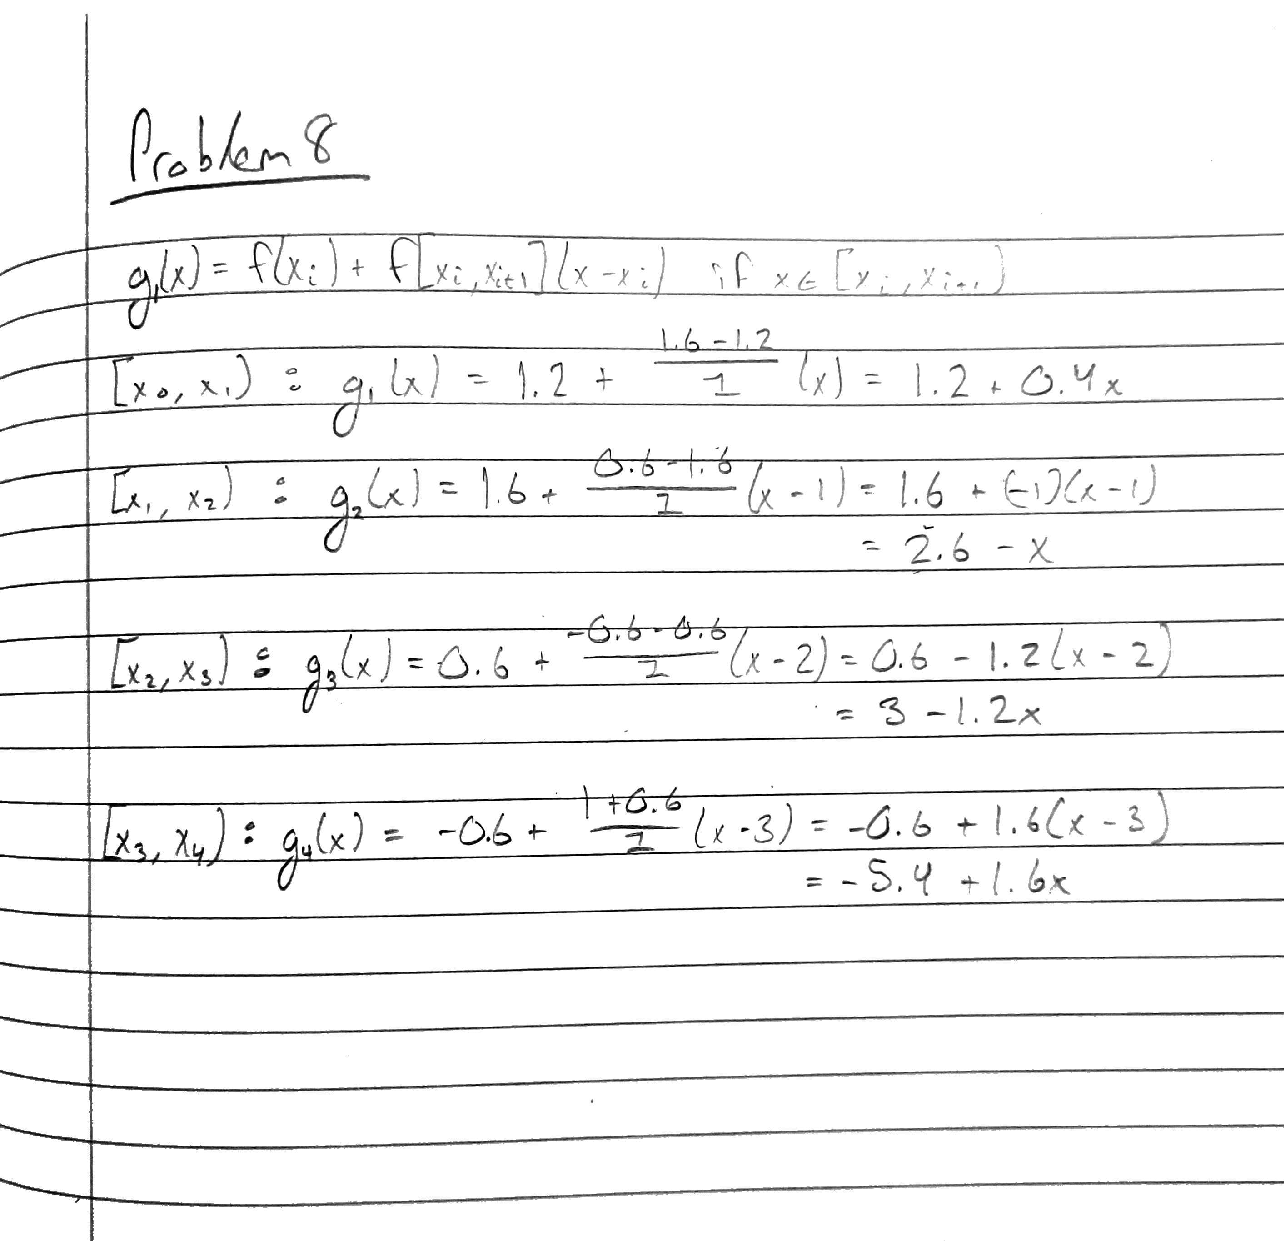
\includepdf[pages=-]{4640_hw1_q8.pdf}

\end{document}
